\documentclass[a4paper]{article}
\usepackage{graphicx}
\usepackage{parskip}
\usepackage{hyperref}
\usepackage{pdflscape}
\usepackage[
    sorting=none
]{biblatex}

\addbibresource{report.bib}
\graphicspath{ {./img/} }

\begin{document}
\title{Computer Architecture Lab 4 Report}
\author{Fabian Wüthrich}
\date{Dezember 2020}
\maketitle

The L2 prefetcher for task 3 is based on the Pangloss prefetcher\cite{pangloss}
presented at the Third Data Prefetching Championship (DPC3)\cite{dpc3}.

Pangloss is a Markov prefetcher\cite{markov-prefetcher} that uses address deltas
to predict complex access patterns. A delta is the difference between two
consecutive addresses. With an initial address and a series of deltas,
a prefetcher is able to reconstruct the address stream. The deltas are limited
by the page boundary as page allocation is not sequential due to, \textit{inter
alia}, security reasons. Thus, the Markov model tracks deltas per page instead
of globally, which enables an efficient representation of the model.

The prefetcher consists of two set-associative caches:
\begin{itemize}
    \item \textbf{Delta Cache} The delta cache is indexed by the current delta.
        Each set holds the most frequent next deltas. The L2 cache works with
        cache line addresses (64-bit) so in a 4KB page we have 64 possible
        offsets i.e. all deltas can be represented by the range (-64, +63] or by
        7 bits.  Additionally, each cache block has a counter which is
          incremented on each cache hit. The counter is used by the replacement
          policy and to calculate the probabilities for subsequent deltas. The
          cache uses a Least Frequently Used (LFU) policy.

    \item \textbf{Page Cache} The page cache keeps track of the last delta per
        page to prevent wrong predictions cause by interleaved pages. The cache
        is indexed by the page address and each cache block includes a tag, the
        previous delta and the previous page offset (used to calculate the
        current delta). The replacement policy is Not Recently Used (NRU).
\end{itemize}

On each L2 lookup, the prefetcher performs the following steps:
\begin{enumerate}
    \item Retrieves the previous delta ($D_{prev}$) and page offset ($O_{prev}$)
        with the current page address from the page cache.

    \item On a page cache hit, it updates the delta cache and the page cache
        with the current delta ($O_{curr} - O_{prev}$).

        On a page cache miss, it stores the current delta and offset in the page
        cache. The delta cache is not updated to prevent wrong predictions.

    \item It traverses the Markov chain (delta cache) from the current delta to
        predict next addresses, until we have as many prefetches as the prefetch
        degree
\end{enumerate}

The last step can be expensive if the prefetcher has to find the best path among
all possible paths. Therefore, the paper proposes a simple heuristic: prefetch
the address occurring from the child deltas with a probability $>1/3$ and
proceed with the highest probable delta for the next iteration, until we count
as many prefetches as the prefetch degree. A prefetch is only issued if the
address lies in the same page.

Figure \ref{fig:performance} compares the prefetchers of each task. The IPC is
normalized to a system without a prefetcher. Pangloss (\texttt{markov} in the
plot) outperforms all prefetchers with an average speedup of 60\% over no
prefetching, 12\% speedup over global history buffer prefetching and 31\%
speedup over feedback directed prefetching. Further performance improvements
might be possible by tuning the cache parameters to the workloads.

\begin{landscape}
\begin{figure}
    \centering
    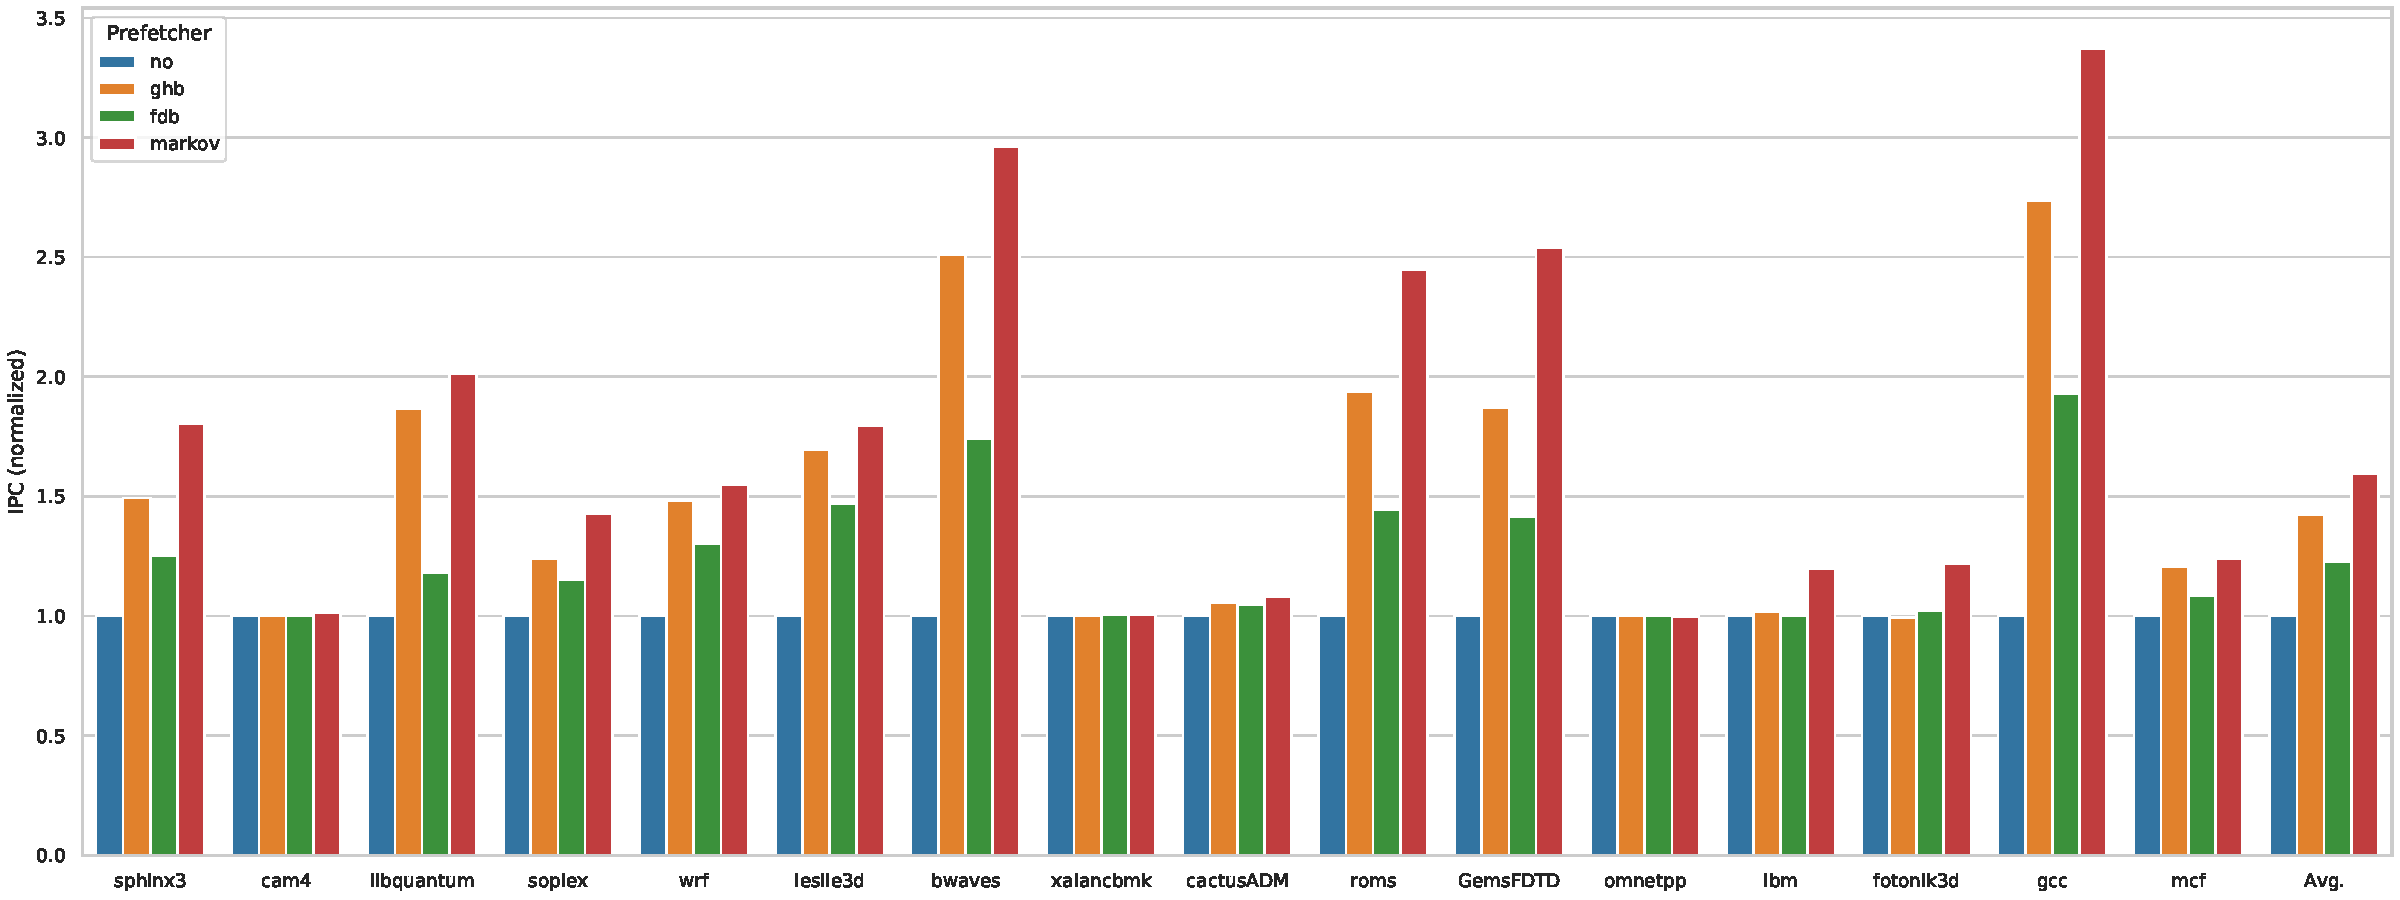
\includegraphics[width=\paperwidth]{plot}
    \caption{Prefetcher Performance}
    \label{fig:performance}
\end{figure}
\end{landscape}

\newpage

\printbibliography

\end{document}
